\documentclass[conference]{IEEEtran}
\IEEEoverridecommandlockouts
% The preceding line is only needed to identify funding in the first footnote. If that is unneeded, please comment it out.
\usepackage[bahasa]{babel}
\usepackage{cite}
\usepackage{amsmath,amssymb,amsfonts}
\usepackage{algorithmic}
\usepackage{graphicx}
\usepackage{textcomp}
\def\BibTeX{{\rm B\kern-.05em{\sc i\kern-.025em b}\kern-.08em
    T\kern-.1667em\lower.7ex\hbox{E}\kern-.125emX}}
\begin{document}

\title{Penerjemah Ensembel Bahasa Indonesia ke Bahasa Inggris dengan Penilaian Tata Bahasa Berbasis Peluang Penguraian\\
}

\author{\IEEEauthorblockN{Stefanus Agus Haryono}
\IEEEauthorblockA{\textit{Sekolah Teknik Elektro dan Informatika} \\
\textit{Institut Teknologi Bandung}\\
Bandung, Indonesia \\
agus@email}
\and
\IEEEauthorblockN{Ratnadira Widyasari}
\IEEEauthorblockA{\textit{Sekolah Teknik Elektro dan Informatika} \\
\textit{Institut Teknologi Bandung}\\
Bandung, Indonesia \\
dira@email}
\and
\IEEEauthorblockN{Muhammad Nizami}
\IEEEauthorblockA{\textit{Sekolah Teknik Elektro dan Informatika} \\
\textit{Institut Teknologi Bandung}\\
Bandung, Indonesia \\
23517044@std.stei.itb.ac.id
}
}

\maketitle

\begin{abstract}
Ringkasan di sini...
\end{abstract}

\begin{IEEEkeywords}
SMT, NMT, ensembel, penilai tata pahasa
\end{IEEEkeywords}

\section{Pendahuluan}

Penerjemah mesin memiliki banyak digunakan baik oleh individu maupun organisasi. Penerjemah mesin biasanya digunakan untuk membantu memahami dokumen oleh non-pengguna bahasa tersebut, atau digunakan juga sebagai tahap awal penerjemahan dokumen untuk selanjutnya diperbaiki oleh penerjemah profesional.

Salah satu prinsip keamanan yang banyak diperhatikan baik oleh pengguna organisasi maupun individu adalah prinsip ketersediaan. Untuk memenuhi prinsip ini, salah satu hal yang dihindari adalah single point of failure. Untuk memberi ilustrasi ancaman ketersediaan dalam penerjemahan mesin: andaikan penyedia layanan penerjemahan mesin “besar” tersebut mengubah syarat dan ketentuan pemakaian seperti pengumpulan data sementara ketentuan pemakaian tersebut tidak sesuai dengan aturan organisasi (misal: aturan kerahasiaan), maka organisasi tersebut tidak dapat menggunakan layanan penerjemahan mesin tersebut. Karenanya, dalam hal penerjemahan mesin, untuk menjamin ketersediaan, dibutuhkan aplikasi yang tidak bergantung kepada penyedia layanan penerjemahan mesin “besar” yang jumlahnya sedikit.

Tiap-tiap organisasi memiliki domain dokumen-dokumen yang diterjemahkannya sendiri. Karenanya, aplikasi penerjemah yang diberikan haruslah mampu dilatih dengan dokumen dari domain tersebut. Aplikasi penerjemah tersebut harus mampu dilatih dengan sumberdaya yang tersedia pada organisasi/pengguna kecil maupun besar.

Salah satu permasalahan penerjemah mesin state-of-the-art SMT dan NMT adalah terkait sumberdaya yang dibutuhkan, baik ukuran dataset maupun sumberdaya komputasi. SMT dan NMT membutuhkan dataset berukuran besar. Pelatihan NMT dengan data besar membutuhkan waktu yang lama. Sementara, aplikasi yang diajukan harus dapat dilatih baik oleh organisasi/pengguna kecil maupun besar dengan sumberdaya yang tersedia.

Apabila dataset yang diberikan kecil, NMT akan banyak menghasilkan kesalahan sintaktik. Kesalahan sintaktik ini, dengan jumlah cukup besar, seringkali juga menyebabkan kalimat menjadi tidak dapat dipahami. Karenanya, dibutuhkan sebuah aplikasi penerjemah yang mampu memberikan penerjemahan yang lebih baik untuk data latih kecil dan sumberdaya komputasi terbatas.

Aplikasi ini dibatasi kepada penerjemahan satu pasangan bahasa dan satu arah saja. Bahasa yang diajukan adalah Bahasa Indonesia ke Bahasa Inggris.

\section{Penerjemah Mesin berbasis Statistik dan Jaringan Syaraf Tiruan}

\section{Penerjemah Mesin Ensembel}

Sistem penerjemah yang diajukan menggabungkan beberapa SMT dan NMT untuk mengatasi banyaknya kesalahan sintaktik pada terjemahan SMT dan NMT. Setelah dilakukan praproses, akan dibuat beberapa kandidat translasi. Translasi terbaik akan dipilih dengan kandidat dengan sintaktik yang dianggap memiliki nilai tertinggi.

Pemilihan translasi terbaik dilakukan untuk memilih kandidat dengan sintaktik yang dianggap memiliki nilai tertinggi. Dalam penilaian yang digunakan untuk pemilihan translasi terbaik, kandidat dengan kesalahan sedikit diberi skor tinggi dan kandidat dengan banyak kesalahan diberi skor rendah.

\section{Penilai Tata Bahasa}

Deskripsi dari struktur sintaktik suatu kalimat dapat dinyatakan dalam struktur frasa, atau disebut juga pohon konstituensi. Diberikan suatu aturan konstituensi (misal CFG), suatu kalimat dapat dinyatakan memenuhi aturan tersebut ataupun tidak\cite{b1}. Sebuah algoritma penguraian berbasis aturan tersebut \cite{b2} yang merupakan kembangan dari algoritma Earley \cite{b3} telah dikembangkan untuk penguraikan pohon kalimat terdekat dari kalimat yang tidak memenuhi aturan tata bahasa yang didefinisikan. Dengan cara ini, kesalahan-kesalahan dalam kalimat dapat dilokalisasi dan dapat dihitung, sehingga kalimat dapat diberi nilai sesuai dengan banyaknya kesalahan tata bahasa di dalamnya.

Persoalan yang muncul dengan pendekatan seperti ini adalah pada aturan dan waktu eksekusi. Dari sisi aturan, sulit untuk mengenumerasi satu per satu aturan tata bahasa untuk bahasa alami dalam bentuk CFG.

Dari sisi waktu eksekusi, algoritma yang diberikan Aho dan Peterson \cite{b2} membangkitkan aturan-aturan tambahan untuk mendeteksi kesalahan tata bahasa. Meski penguraiannya dinyatakan berkompleksitas kubik terhadap panjang kalimat, Aho dan Peterson tidak menjelaskan kompleksitas waktu terhadap ukuran CFG yang diberikan. Dari hasil eksekusi implementasi algoritma tersebut\footnote{https://github.com/muhammadnizami/error-correcting-earley-parser-demo}, didapati bahwa dengan jumlah aturan produksi nonterminal lebih dari 4 dan aturan produksi terminal lebih dari 5, waktu eksekusi menjadi tidak praktikal untuk digunakan.

Penilaian tata bahasa untuk memilih di antara kandidat terjemahan tidak membutuhkan untuk melokalisasi titik kesalahan tata bahasa. Dengan mengabaikan titik kesalahan tata bahasa dan fokus kepada seberapa mungkin sebuah kalimat memiliki kesalahan tata bahasa, waktu eksekusi penilaian tata bahasa dapat dipercepat. Wagner dan Foster \cite{b4} menunjukkan adanya keterhubungan antara peluang penguraian dengan pengurai probabilistik dengan kesalahan tata bahasa dalam kalimat. Dalam Wagner dan Foster\cite{b4}, ditunjukkan bahwa pemberian kesalahan pada kalimat umumnya menyebabkan penurunan peluang penguraian.

\begin{figure}[h]
\centerline{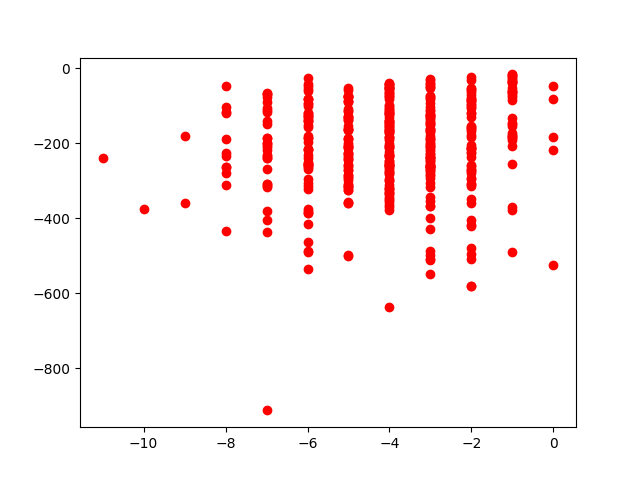
\includegraphics[width=\columnwidth]{figures/figscoretoparseprob.png}}
\caption{Perbandingan skor negatif jumlah kesalahan (sumbu horisontal) kalimat terhadap skor penguraian (sumbu vertikal) dengan BLLIPParser. Data diambil dari data latih sintektik dari BNC dengan pemberian kesalahan GenERRate yang dimodifikasi}
\label{figscoretoparseprob}
\end{figure}

Hubungan antara jumlah kesalahan dalam kalimat terlihat pada gambar \ref{figscoretoparseprob}. Dalam gambar ini, terlihat bahwa pada umumnya, semakin sedikit kesalahan maka semakin tinggi skor penguraiannya. Di sini, hubungan tidak terlalu terlihat karena terdapat bias panjang kalimat. Semakin panjang kalimat, skor penguraian semakin rendah. Hal ini terlihat pada gambar \ref{figlentoparseprob}.

\begin{figure}[h]
\centerline{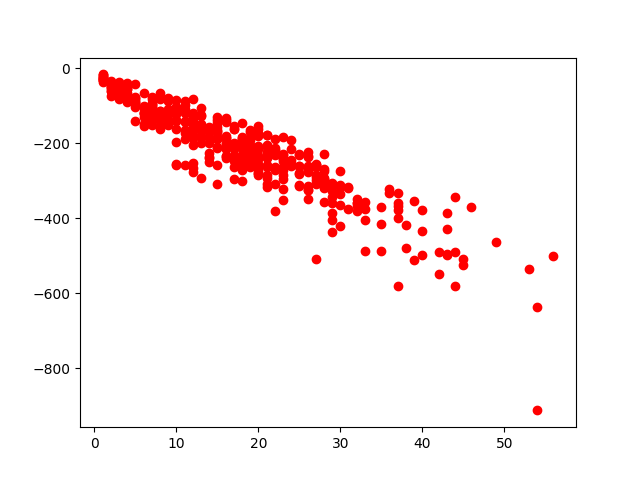
\includegraphics[width=\columnwidth]{figures/figlentoparseprob.png}}
\caption{Perbandingan panjang kalimat (sumbu horisontal) terhadap skor penguraian (sumbu vertikal) dengan BLLIPParser. Data diambil dari data latih sintektik dari BNC dengan pemberian kesalahan GenERRate yang dimodifikasi}
\label{figlentoparseprob}
\end{figure}

Untuk itu, dilakukan transformasi di mana skor penguraian dibagi dengan panjang kalimat. Hal ini dapat mengurangi bias panjang kalimat, sebagaimana terlihat pada gambar \ref{figlentoparseprobtransformed}. Terlihat bahwa panjang kalimat tidak lagi terlalu memengaruhi skor penguraian.

\begin{figure}[h]
\centerline{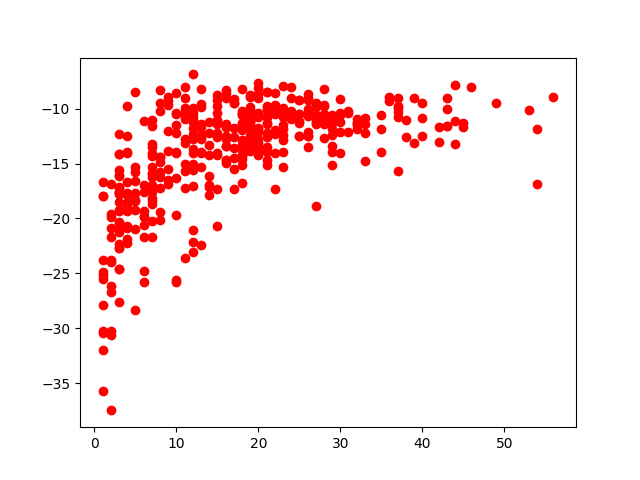
\includegraphics[width=\columnwidth]{figures/figlentoparseprobtransformed.png}}
\caption{Perbandingan panjang kalimat (sumbu horisontal) terhadap skor penguraian (sumbu vertikal) dengan BLLIPParser yang ditransformasi. Data diambil dari data latih sintektik dari BNC dengan pemberian kesalahan GenERRate yang dimodifikasi}
\label{figlentoparseprobtransformed}
\end{figure}

Dengan demikian, hubungan antara skor negatif jumlah kesalahan dan skor penguraian menjadi lebih tampak. Hal ini terlihat pada gambar \ref{figscoretoparseprobtransformed}. Terlihat bahwa pada umumnya, semakin sedikit kesalahan maka skor penguraian menjadi semakin besar. Meski terdapat beberapa kasus di mana skor penguraian rendah dan jumlah kesalahan sedikit, namun kasus ini berjumlah sedikit dan hanya berupa pencilan saja.

\begin{figure}[h]
\centerline{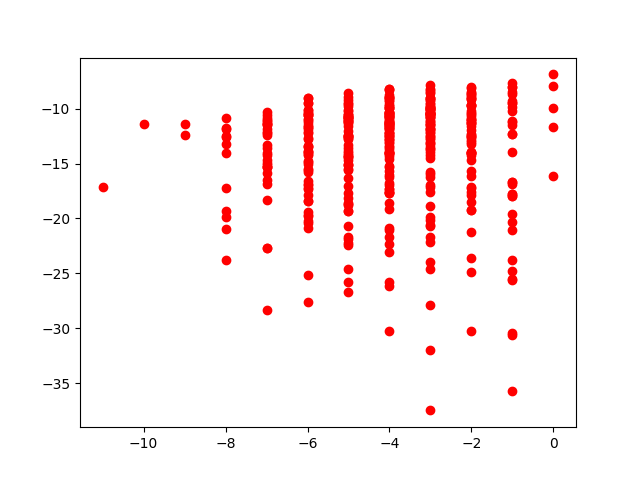
\includegraphics[width=\columnwidth]{figures/figscoretoparseprobtransformed.png}}
\caption{Perbandingan skor negatif jumlah kesalahan (sumbu horisontal) kalimat terhadap skor penguraian (sumbu vertikal) dengan BLLIPParser yang ditransformasi. Data diambil dari data latih sintektik dari BNC dengan pemberian kesalahan GenERRate yang dimodifikasi}
\label{figscoretoparseprobtransformed}
\end{figure}

Meski peluang penguraian saja dapat menunjukkan kemungkinan kesalahan pada kalimat, namun ia tidak secara eksplisit menyatakan suatu kalimat kandidat terjemahan lebih baik daripada kalimat lain secara sintaktik. Karenanya, selain penilaian tanpa regresi (langsung dari peluang penguraian), dicobakan pula penilaian dengan regresi.

Dengan demikian, penilaian tata bahasa dilakukan dengan menggunakan peluang penguraian dari pengurai konstituensi probabilistik. Dari peluang penguraian ini dilakukan regresi terhadap skor penguraian yang tersedia dalam data latih. Skor penguraian adalah negatif dari banyaknya kesalahan dalam kalimat.
Pengurai konstituensi probabilistik yang digunakan adalah BLLIPParser\cite{b5}\cite{b6}\cite{b7}\cite{b8}, dengan model pralatih WSJ+Gigaword-v2. Pengurai ini menggunakan teknik coarse-to-fine n-best parsing dengan reranking. Model pralatih ini dilatih menggunakan entropi maksimum dan pelatihan-diri.
Terdapat beberapa pilihan untuk teknik regresi yang digunakan:

\begin{itemize}
\item Tanpa regresi
\item Regresi linear
\item Regresi MLP
\end{itemize}

Peubah terikat (target) dari regresi ini adalah skor grammar kalimat. Peubah bebas (fitur) dari regresi ini diambil dari peluang penguraian dari n-buah penguraian terbaik. Peluang penguraian tersebut dapat langsung digunakan sebagai fitur ataupun ditransformasi dengan cara dibagi dengan panjang kalimat.

\section{Eksperimen}

Eksperimen ini terdiri dari eksperimen penilai tata bahasa dan eksperimen translasi. Eksperimen tiap-tiap modul translasi akan dijelaskan bersamaan dengan eksperimen translasi gabungan.

\subsection{Eksperimen Penilai Tata Bahasa}

Data yang digunakan untuk eksperimen merupakan pasangan data (Kalimat, Jumlah Kesalahan) yang kemudian dalam program akan ditransformasi menjadi pasangan data (Kalimat, Skor) di mana skor adalah negatif dari jumlah kesalahan. 
Data yang digunakan merupakan data sintetik berupa sampel data kalimat yang diberi kesalahan. Kalimat yang digunakan merupakan sampel 823 kalimat dari British National Corpus\cite{b9}. Kalimat diberi kesalahan dengan cara yang diberikan dengan cara mirip dengan GenERRate Foster dan Anderson\cite{b10}:
\begin{itemize}
\item Penghapusan kata
\item Penyisipan kata
\item Pemindahan kata
\item Penggantian kata
\end{itemize}
Dari teknik pembangkitan data sintetik GenERRate\cite{b10}, dilakukan modifikasi yang memungkinkan sebuah kalimat untuk memiliki beberapa kesalahan sintaktik. Satu kalimat akan diberikan kesalahan untuk tiap-tiap spesifikasi kesalahan secara berurutan dalam peluang yang dispesifikasikan. Spesifikasi kesalahan yang digunakan adalah keempat kesalahan tersebut memiliki peluang masing-masing 0,1 dan diulang sebanyak 12 kali.

Dari 823 kalimat yang ada, 423 kalimat digunakan untuk melatih model dan 400 digunakan untuk pengujian. Untuk teknik tanpa regresi, tidak dilakukan pelatihan. Untuk teknik regresi linear dan regresi MLP, dilakukan pelatihan dan pengujian dengan variasi parameter banyaknya pohon penguraian 1,3, dan 5 serta parameter skor penguraian tanpa transformasi dan dengan transformasi. Ukuran kinerja yang digunakan adalah koefisien korelasi. Hasil eksperimen ini terlihat pada Tabel \ref{tabeksperimenscoring}.

\begin{table}[h]
\caption{Hasil eksperimen penilaian tata bahasa}
\begin{center}
\begin{tabular}{|c|c|c|}
\hline
\textbf{Teknik}&\multicolumn{2}{|c|}{\textbf{Koefisien Korelasi}} \\
\cline{2-3} 
 & \textbf{\textit{Data Latih}}& \textbf{\textit{Data Uji}} \\
\hline
Tanpa Regresi& 0.0350564& 0.2315319 \\
Regresi Linear, tanpa transformasi, 1 pohon& 0.2844588&
0.3131186  \\
Regresi Linear, tanpa transformasi, 3 pohon&0.2844588 & 0.3131186 \\
Regresi Linear, tanpa transformasi, 5 pohon&0.2844588 & 0.3131186 \\
Regresi Linear, transformasi, 1 pohon&0.2844588 & 0.3131186 \\
Regresi Linear, transformasi, 3 pohon&0.2844588 &0.3131186  \\
Regresi Linear, transformasi, 5 pohon&0.2844588 & 0.3131186 \\
MLP, tanpa transformasi, 1 pohon&0.0119836 & 0.2214019 \\
MLP, tanpa transformasi, 3 pohon&0.0025130 &0.2113910  \\
MLP, tanpa transformasi, 5 pohon&0.0211636 & 0.2262849 \\
MLP, transformasi, 1 pohon&0.0879850 &0.2670922  \\
MLP, transformasi, 3 pohon&-0.0038575 &0.2014690  \\
MLP, transformasi, 5 pohon&-0.0202959 &0.1961423  \\
\hline
\end{tabular}
\label{tabeksperimenscoring}
\end{center}
\end{table}

Koefisien korelasi tertinggi didapat dengan teknik regresi linear. Tidak ada perbedaan koefisien korelasi pada teknik dengan transformasi maupun tanpa transformasi untuk teknik regresi linear. Begitu pula jumlah pohon penguraian tidak memengaruhi kinerja Grammar Scoring dengan teknik regresi linear. Adapun untuk regresi dengan MLP, perbedaan transformasi dan juga banyaknya pohon penguraian yang digunakan memengaruhi kinerja yang didapatkan. Parameter yang berbeda menghasilkan kinerja berbeda, meski semuanya tidak mampu mengungguli kinerja regresi linear.

Koefisien korelasi yang didapatkan masih rendah, yaitu paling tinggi sebesar 0.31311855. Angka kinerja yang rendah untuk data latih menunjukkan bahwa permasalahannya bukanlah kekurangan data latih. Rendahnya korelasi ini disebabkan karena pengujian dilakukan kepada data uji yang memiliki kalimat-kalimat beragam. Kalimat-kalimat beragam akan memiliki peluang penguraian yang beragam pula, dan akibatnya pada saat diberikan regresi akan didapatkan standar skor yang beragam.

\begin{table}[h]
\caption{Contoh nilai yang diberikan kepada kalimat yang tidak mirip}
\begin{center}
\begin{tabular}{|c|p{4cm}|c|c|}
\hline
\textbf{No}&\textbf{Kalimat}&\textbf{\textit{Error}}&\textbf{Skor yang Diberikan}\\
\hline
1&Did you know ?&0&-5.5259\\
\hline
2&You can do it on your own or you can get together with family and friends . &0&-5.0638\\
\hline
3&Why not have a clear out ?&0&-7.5650\\
\hline
4&Do n't plan on selling too much at more than 10p an item .&0&-7.4124\\
\hline
5&3 .&0&-7.0221\\
\hline
6&This is an example sentence .&0&-9.0859\\
\hline

\end{tabular}
\label{tabeksperimenscoringnotsimilarexample}
\end{center}
\end{table}

Semua kalimat no. 1 s.d. 5 dalam tabel \ref{tabeksperimenscoringnotsimilarexample} berasal dari korpus BNC tanpa diberi kesalahan. Kalimat no. 6 adalah kalimat yang dibuat sebagai contoh. Meski kalimat-kalimat tersebut sama-sama tidak diberi kesalahan, skor yang diberikan memiliki jangkauan yang cukup luas, dari -5 hingga -9. Dalam data uji yang digunakan, kalimat-kalimat berkesalahan yang digunakan berasal dari kalimat-kalimat BNC yang bermacam-macam. Akibatnya, nilai korelasi menjadi rendah.

Yang menjadi perhatian utama adalah bagaimana kinerja penilai tata bahasa terhadap kalimat-kalimat yang mirip. Hal ini karena dalam pemilihan kandidat translasi, kandidat-kandidat berasal dari penerjemahan kalimat yang sama.


\begin{table}[h]
\caption{Contoh nilai yang diberikan kepada kalimat yang mirip}
\begin{center}
\begin{tabular}{|c|p{4cm}|c|r|}
\hline
\textbf{No}&\textbf{Kalimat}&\textbf{\textit{Error}}&\textbf{Skor yang Diberikan}\\
\hline
1&This is an example sentence .&0&-9.085\\
\hline
2&This are an example sentence . &1&-11.542\\
\hline
3&This did was it example sentences .&3&-11.728\\
\hline
4&This an example sentence .&1&-12.674\\
\hline

\end{tabular}
\label{tabeksperimenscoringsimilarexample}
\end{center}
\end{table}

Dalam tabel \ref{tabeksperimenscoringsimilarexample}, diberikan beberapa contoh kalimat yang mirip, dengan perbedaan terletak pada kesalahan tata bahasa. Kalimat pertama merupakan kalimat tanpa kesalahan. Kalimat kedua merupakan kalimat pertama dengan tambahan kesalahan penggantian ‘is’ menjadi ‘are’. Kalimat ketiga memiliki kesalahan penggantian ‘are’ menjadi ‘was’, ‘sentence’ menjadi ‘sentences’, dan kesalahan penyisipan ‘did’. Kalimat keempat memiliki kesalahan penghapusan ‘is’.

Secara umum, kalimat tanpa kesalahan diberikan skor prediksi paling tinggi. Kalimat yang memiliki kesalahan lebih banyak umumnya diberi skor prediksi yang lebih rendah (lihat kalimat no. 1, 2, dan 3). Meski demikian, masih ada beberapa kasus di mana kalimat yang memiliki kesalahan sedikit diberi skor lebih rendah daripada kalimat yang memiliki banyak kesalahan (lihat kalimat no. 3 dan 4).

\subsection{Eksperimen Penerjemah}

\section{Kesimpulan dan Saran}

\section*{Ucapan Terima Kasih}

\begin{thebibliography}{00}
\bibitem{b1} Chomsky, Noam (Sep 1956), ``Three models for the description of language,'' Information Theory, IEEE Transactions, 2 (3): 113--124
\bibitem{b2} Alfred V. Aho, ``A Minimum Distance Error-Correcting Parser for Context-Free Languages,'' in SIAM Journal on Computing 1(4):305-312 · December 1972
\bibitem{b3}Earley, Jay (1970), ``an efficient context-free parsing algorithm'', Communications of the ACM, 13 (2): 94--102
\bibitem{b4} J. Wagner and J. Foster, ``The effect of correcting grammatical errors on parse probabilities,'' in Proceedings of the 11th International Conference on Parsing Technologies (IWPT), pp 176--179,. Paris, October 2009
\bibitem{b5} Do Kook Choe, David McClosky, and Eugene Charniak. ``Syntactic Parse Fusion.'' Proceedings of the Conference on Empirical Methods in Natural Language Processing (EMNLP 2015), 2015.
\bibitem{b6} David McClosky, Eugene Charniak, and Mark Johnson. ``Effective Self-Training for Parsing.'' Proceedings of the Conference on Human Language Technology and North American chapter of the Association for Computational Linguistics (HLT-NAACL 2006), 2006.
\bibitem{b7} Eugene Charniak and Mark Johnson. ``Coarse-to-fine n-best parsing and MaxEnt discriminative reranking.'' Proceedings of the 43rd Annual Meeting on Association for Computational Linguistics. Association for Computational Linguistics, 2005.
\bibitem{b8} Eugene Charniak. ``A maximum-entropy-inspired parser.'' Proceedings of the 1st North American chapter of the Association for Computational Linguistics conference. Association for Computational Linguistics, 2000.
\bibitem{b9} The British National Corpus, version 3 (BNC XML Edition). 2007. Distributed by Bodleian Libraries, University of Oxford, on behalf of the BNC Consortium. URL: http://www.natcorp.ox.ac.uk/
\bibitem{b10} Jennifer Foster and Oistein E. Andersen, 2009. GenERRate: Generating Errors for Use in Grammatical Error Detection. Proceedings of the NAACL Workshop on Innovative Use of NLP for Building Educational Applications, Boulder, Colorado.
\end{thebibliography}


\end{document}
